% Matteo Kumar
% PPB2 AFM
%Grundlagen

\chapter{Grundlagen}

\section{FRET}

Förster-Resonanzenergietransfer ist ein Prozess des Energietransfers. Dabei gibt ein Donor und einen Akzeptor. Der Donor gibt dabei über Dipol-Dipol-Wechselwirkung 
Energie an den Akzeptor ab – und das strahlungsfrei.
Damit FRET auftritt müssen bestimmte Voraussetzungen erfüllt sein. Diese wären, dass sich das Emissionsspektrum des Donors und das Absorptionsspektrum des Akzeptors überlappen wie in  
Abbildung \ref{bild:FRETSpektrum}.

\begin{figure}[h]
    \centering
    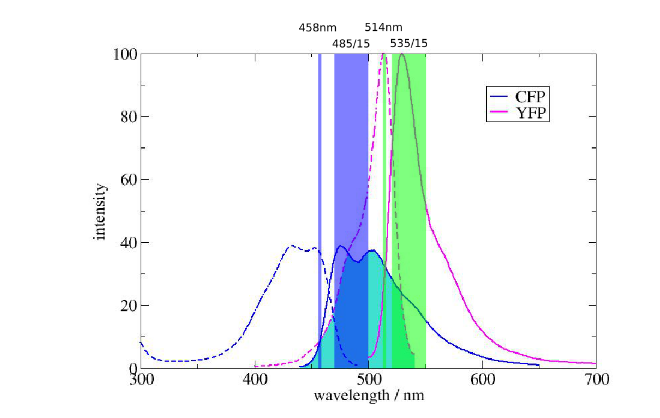
\includegraphics[width = 10cm]{Bilder/Grundlagen/FRETSpektrum.png}
    \caption{Emissionsspektrum/Absorptionsspektrum von CPF/YFP}
    \label{bild:FRETSpektrum}
\end{figure}

Sollte dies der Fall sein und der Abstand klein genug sein, dann tritt FRET auf. \\
Der Abstand muss klein genug sein, da die FRET-Effizienz\\


\begin{equation}
    E = \frac{1}{1+\frac{r^6}{R_0^6}}
\end{equation}
ist. Dabei bezeichnet $R_0$ den Försterradius und $r$ den Abstand der beiden Moleküle. Man sieht seht schön, dass $E = 1/2$ für $r = R_0$. Das ist auch die 
Definition des Försterradiuses: Die Hälfte der einfallenden Photonen, die vom Donor absorbiert werden, werden über FRET auf den Akzeptor übertragen.\\
Der Försterradius liegt normalerweise im Millimeterbereich, da die Dipol-Dipol-Wechselwirkung sehr kurzreichweitig ist. Daher kommt auch die sechste Potenz unter dem Bruchstrich.\\
Wichig ist noch, dass ein Teil der Energie als Vibration bei dem emittierenden Molekül bleibt. Daher ist die emittierte Strahlungen energieärmer als die absorbierte Strahlungen.


\section{Bleichung}